\documentclass[11pt]{article} 

\setlength{\parindent}{0pt}
\usepackage{xltxtra}
\usepackage{hyperref}
\hypersetup{hidelinks}
\usepackage{url}
\urlstyle{tt}
\usepackage{xcolor}
\definecolor{CVBlue}{RGB}{23,110,191}
\usepackage{calc}
\usepackage{graphicx}
\usepackage{tikz} 
\usetikzlibrary{calc}
\usepackage{fontspec}
\usepackage{xeCJK}
\usepackage{enumitem}

% --- 重要修改 1: 注释掉 \CJKsetecglue{} ---
% 在 GitHub Actions 的 Linux 环境下，此命令常导致 xelatex 崩溃 (Return Code 1)
% \CJKsetecglue{} 

% --- 字体设置 ---
\setmainfont[Path = fonts/Main/, Extension = .otf, BoldFont = texgyretermes-bold.otf]{texgyretermes-regular.otf}
\setCJKmainfont[Path = fonts/hansans/, Extension = .ttf, BoldFont = NotoSansSC-Bold.ttf]{NotoSansSC-Regular.otf}
\setlist[itemize]{nosep, topsep=0pt, partopsep=0pt, leftmargin=*}
% --- A4纸，上下左右边距 ---
\usepackage[
    a4paper,
    left=1.2cm,
    right=1.2cm,
    top=1.0cm,    % 从 1.5cm 降至 1.0cm
    bottom=0.8cm, % 从 1.0cm 降至 0.8cm
    nohead
]{geometry}

\renewcommand{\baselinestretch}{1.3} 

\usepackage{titlesec}
\titleformat{\section}{\Large\bfseries\raggedright}{}{0em}{}[{\color{CVBlue}\titlerule}]
\titlespacing*{\section}{0cm}{*1.4}{*1.0}

\usepackage{fontawesome}

\begin{document}
\pagenumbering{gobble}

% =======================================================================
%%%% 重要修改 2: 图片插入代码优化 %%%%
% 确保 picture.jpg 位于根目录，建议文件大小控制在 500KB 以内以避免 Actions 内存溢出
\begin{tikzpicture}[remember picture, overlay]
    \node[anchor = north east] at ($(current page.north east)+(-1.5cm,-1.5cm)$) {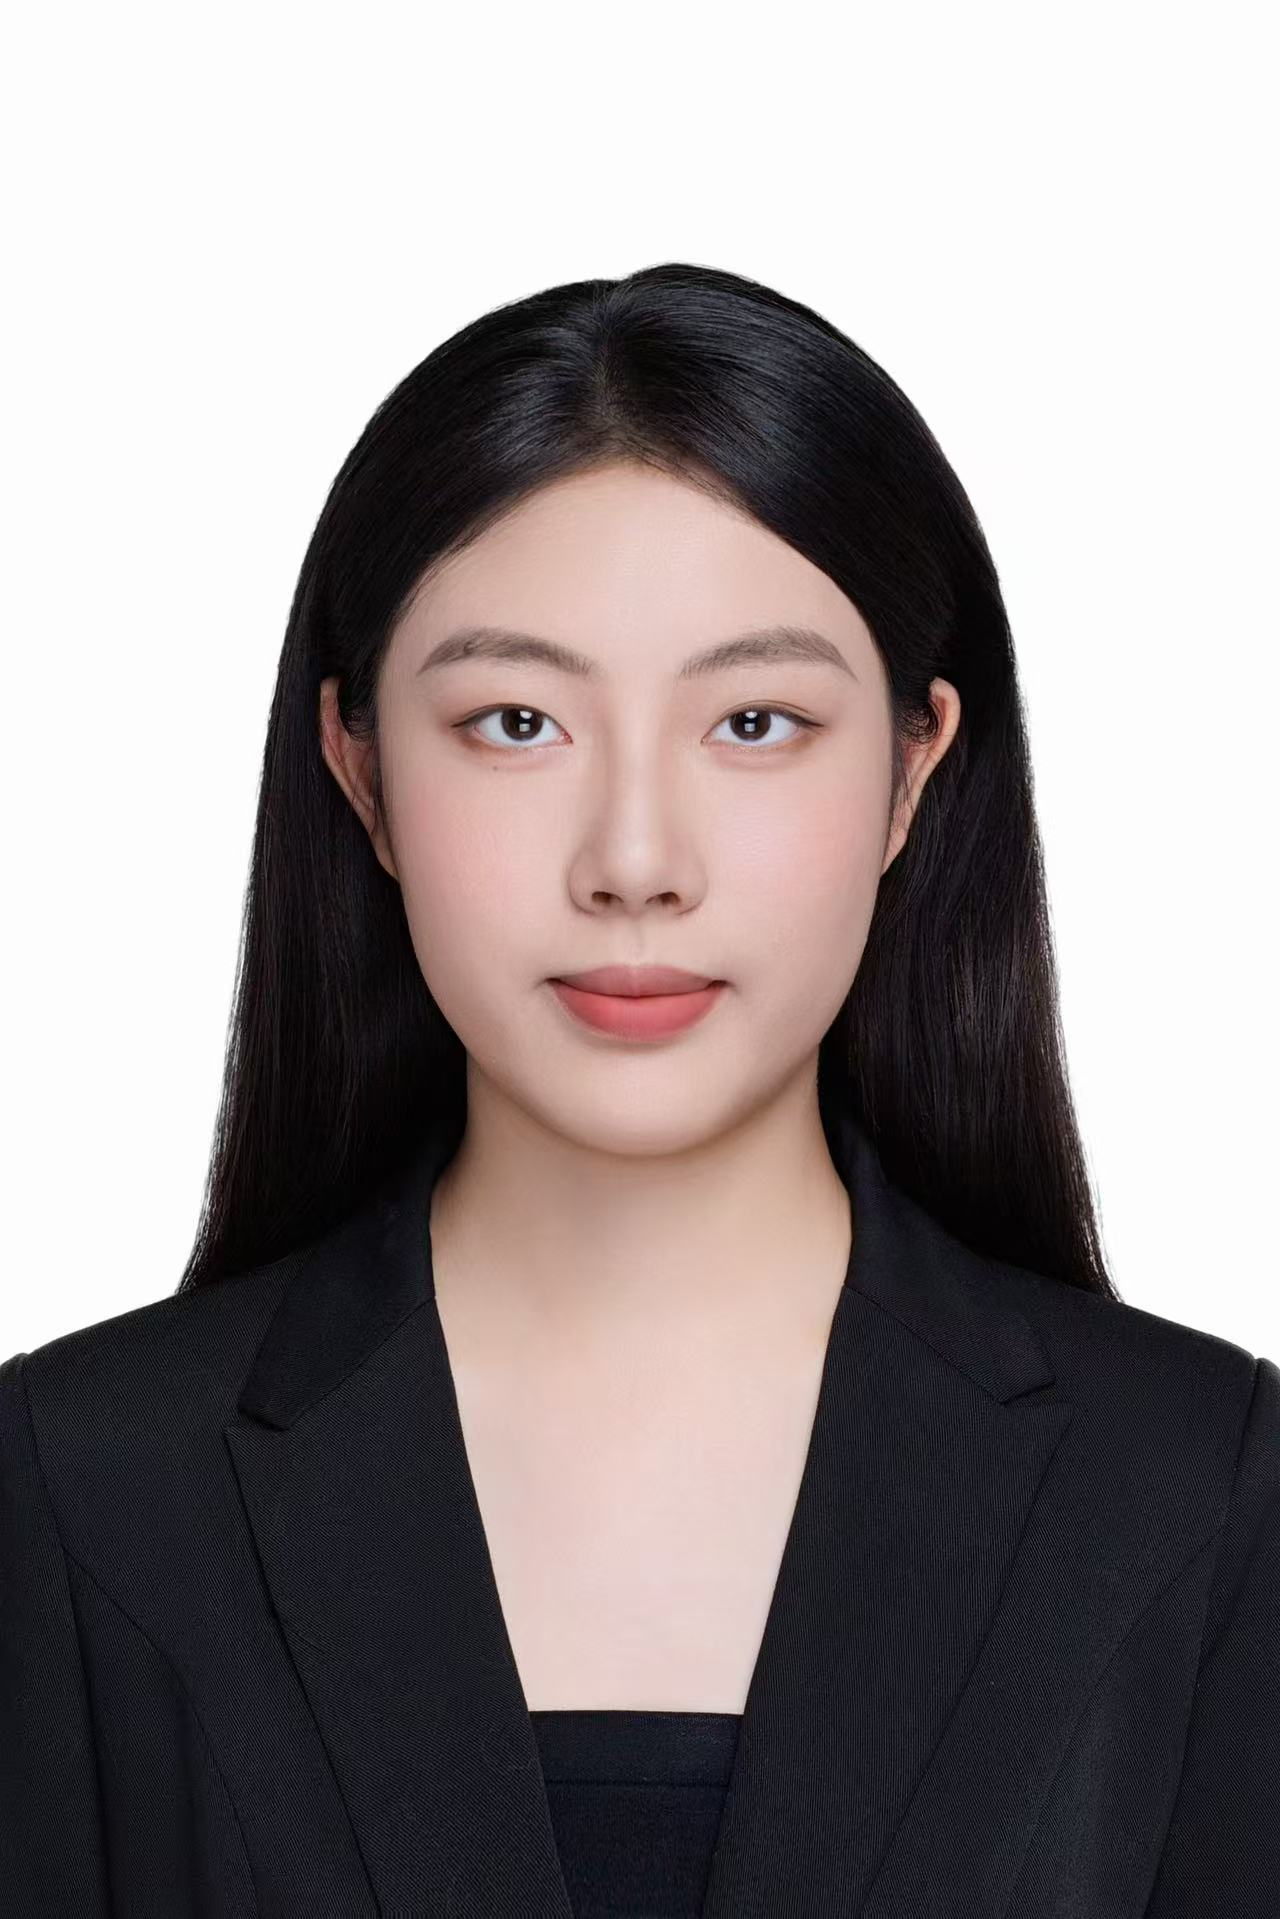
\includegraphics[height=3.2cm]{picture.jpg}};
\end{tikzpicture}
% =======================================================================

% --- 个人信息 ---
\vspace{1.0em} 
{\LARGE\bfseries{谢宛值}} \hfill \\ 
\normalsize{\faPhone\ 19033955091 \quad \faEnvelopeO\ \href{mailto:3240105510@zju.edu.cn}{3240105510@zju.edu.cn}} \hfill \\ 

\vspace{0.8em} 

% --- 教育背景 ---
\section{\faGraduationCap\ 教育背景} 
\textbf{浙江大学} \hfill 2024.09 -- 至今 \\
软件工程\quad 本科（大二） \hfill \textbf{均绩：4.36}
\begin{itemize}[nosep]
    \item \textbf{核心课程}：C程序设计(\textbf{5.0})、面向对象程序设计(\textbf{4.8})、现代软件工程实践(\textbf{5.0})、数据结构基础(\textbf{4.8})。
    \item \textbf{学术交流}：大一暑期赴\textbf{香港大学}进行为期一周的交流学习，深入研讨 6G 通信技术前沿。
\end{itemize}

% --- 科研与项目经历 ---
\section{\faUsers\ 科研与项目经历}

\textbf{SRTP 核心科研：面向多模态大模型推理能力评测的学科竞赛题目合成} \hfill 2026.04 -- 至今 \\
\textit{角色：核心科研成员 \hfill 指导成果：核心物理方向论文预计于 2026 年 5 月发表}
\begin{itemize}[nosep]
    \item \textbf{前沿调研与基准体系构建}：系统调研 LLM 科学推理领域进展，梳理整合 \textbf{SciBench, GPQA, OlympiadBench} 等高难度评测基准；深度分析提炼 \textbf{Evol-Instruct, Generator-Verifier} 等核心 Baseline 对比方案，为课题组的题目合成与能力评估确立了科学的对比标准。
    \item \textbf{合成数据集测评与校验}：在课题组前期被 \textbf{ICML 2026 (MathLEGO)} 录用的方法基础上，负责对生成的复杂物理竞赛题集进行多维度测评。验证基于“同源耦合法、单体变异法及自进化机制”生成题目的有效性，排查大模型的逻辑谬误并探索其多步推理边界。
    \item \textbf{自动化合成管线开发 (Python)}：独立负责化学与生物学科的数据拓展，编写高效的自动化数据处理与爬虫脚本。基于 \textbf{o3-mini} 模型 API 与少样本提示词工程，以 200 余个竞赛级核心考点（如 IChO 理论）为驱动，全自动合成并校验了 1000+ 道结合“深空探测”等极端科研场景的高难度试题数据集。
    \item \textbf{学术论文撰写}：梳理大语言模型在硬核科学问题上的性能表现与数据集构建发展脉络，独立承担团队待发表核心物理方向论文中 \textbf{Related Work} 部分的撰写。
\end{itemize}

\vspace{0.6em}
\textbf{LLM 安全与内容风控研究（课题组）} \hfill 2024.12 -- 2025.12 \\
\textit{简述：参与大模型安全可信研究，负责收集对抗性 Prompt，测试并探索扩散模型（Diffusion Models）在图像生成内容过滤及合规性方面的鲁棒性边界。}

\vspace{0.6em}
\textbf{现代软件工程综合实践：区块链系统模拟与分析} \hfill 2025.08 \\
\textit{简述：利用 Python/C++ 实现了基于 UTXO 模型与非对称加密的区块链交易全链路模拟，并完成多类典型智能合约（如重入攻击）的安全审计，获评 5.0 满绩。}

\vspace{0.6em}
\textbf{求是潮技术开发部 - Web 前端工程实践} \hfill 2025.03 -- 2025.12 \\
\textit{简述：运用 HTML/CSS/JS 原生开发及 Git 协同工作流程，负责校内知名社区平台前端交互组件的迭代开发与日常维护。}

% --- 技能与获奖 ---
\section{\faCogs\ 技术栈 \& 获奖情况}
\begin{itemize}[nosep]
    \item \textbf{编程语言与技术}：熟练掌握 \textbf{Python, C/C++}；熟悉大模型 Prompt 工程、API 自动化调用及数据处理；熟悉前端基础。
    \item \textbf{前沿探索}：自学机器学习与神经网络，正深入研读脑机接口 (BCI) 与 AI4Science 领域论文。
    \item \textbf{获奖荣誉}：浙江大学\textbf{三等奖学金}，浙江省大学生物理创新竞赛（理论） \textbf{三等奖}。
    \item \textbf{英语水平}：\textbf{CET-4: 581分}（优秀），\textbf{CET-6: 513分}，具备良好的英文论文阅读与学术写作能力。
\end{itemize}

% --- 综合素质 ---
\section{\faInfoCircle\ 综合素质}
\begin{itemize}[nosep]
    \item \textbf{学生工作}：云峰学风建设与学业指导中心 \textbf{学术文化部副部长}，负责大型学术活动策划；班级宣传委员，荣获优秀班干部。
    \item \textbf{自驱力}：对前沿技术具备强烈的自驱力与好奇心，拥有快速的自学能力和扎实的代码动手能力。
    \item \textbf{社会实践工作}：大一暑假参加金华市西联乡小学支教，大二寒假担任队长组织红色研学实践活动。
\end{itemize}

\end{document}
